\documentclass[11pt]{article}
\usepackage[a4paper,margin=26mm]{geometry}
\usepackage[T1]{fontenc}
\usepackage{lmodern}
\usepackage{amsmath,amssymb,amsthm}
\usepackage{microtype}
\usepackage{array}
\usepackage{tikz}
\usepackage{xurl}
\usepackage{hyperref}
\hypersetup{colorlinks=true,linkcolor=blue,urlcolor=blue,citecolor=blue,
 pdftitle={The generalized Wilf conjecture for semigroups graded by a two-generated numerical semigroup},
 pdfauthor={Horace Dong}}
\newtheorem{theorem}{Theorem}
\newtheorem{lemma}{Lemma}
\newtheorem{proposition}{Proposition}
\newtheorem{corollary}{Corollary}
\theoremstyle{definition}
\newtheorem{definition}{Definition}
\theoremstyle{remark}
\newtheorem{remark}{Remark}
\newcommand{\repoversion}{1.25.0}
\setlength{\emergencystretch}{1.5em}
\newcommand{\N}{\mathbb N}
\newcommand{\Bd}[2]{B_{#1}(#2)}

\title{The generalized Wilf conjecture for semigroups\\ graded by a two-generated numerical semigroup}
\author{Horace Dong\\ \small Independent researcher\\
\small\texttt{maxwelldhx@gmail.com}\\
\small ORCID: \href{https://orcid.org/0009-0002-7554-7548}{0009-0002-7554-7548}}
\date{22 November 2026}
\begin{document}
\maketitle

\begin{abstract}
A generalized numerical semigroup is a submonoid $S$ of $\N^d$ with finite
complement. Cisto, DiPasquale, Failla, Flores, Peterson and Utano conjectured
that every such $S$ satisfies $e(S)\,n(S)\ge d\,c(S)$, where $e(S)$ is the
number of minimal generators and $n(S)$ and $c(S)$ count the elements of $S$,
respectively of $\N^d$, that lie below some gap. For a numerical semigroup
$T$, the $T$-graded semigroup consists of the points of $\N^d$ whose
coordinate sum lies in $T$. Cisto and Navarra proved the conjecture for
$T=\langle 2,b\rangle$ with $b\ge5$ odd and stated that it remains open for
$T=\langle a,b\rangle$ with $2<a<b$. Bhardwaj, Cisto and Deshpande recently
proved it in dimension $d=2$, and in dimension $d\ge3$ under a condition that
requires $b$ to be large compared with $a$ and $d$. We prove the inequality for
every $d\ge1$ and every two-generated numerical semigroup $T$; the case not covered
by these results is $d\ge3$, $a\ge3$ with that condition failing. The proof bounds $n(S)$ from
below by the single layer of total degree $F(T)-1$, where $F(T)$ is the
Frobenius number of $T$, and compares it directly with the exact value of $c(S)$. The result is formally verified in Lean~4. The
proofs were found and formalized by AI agents working under the author's
direction; their role is described at the end of the paper.
\end{abstract}

\section{Introduction}

Let $\N=\{0,1,2,\dots\}$ and $d\ge1$. A \emph{generalized numerical semigroup}
(GNS) is a submonoid $S$ of $(\N^d,+)$ such that the set of gaps
$H(S)=\N^d\setminus S$ is finite; for $d=1$ these are the numerical semigroups.
Every GNS has a unique minimal system of generators $G(S)$ (see~\cite[§2]{cn}), and
$e(S)=|G(S)|$ is its \emph{embedding dimension}. Let $\le$ be the coordinatewise
partial order on $\N^d$, so that $x\le y$ if and only if $y-x\in\N^d$. Following
Cisto, DiPasquale, Failla, Flores, Peterson and Utano~\cite{cdffpu}, put
\[
C(S)=\{x\in\N^d : x\le h \text{ for some } h\in H(S)\},\qquad
N(S)=C(S)\cap S,
\]
$c(S)=|C(S)|$, $n(S)=|N(S)|$ and $g(S)=|H(S)|$. A point below several gaps is
counted once, and every gap lies in $C(S)$, so $c(S)=n(S)+g(S)$. In~\cite{cdffpu}
they proposed the following generalization of Wilf's conjecture~\cite{wilf}; we
quote it in the form of~\cite[Conjecture~2.1]{cn}.

\begin{quote}
\textbf{Generalized Wilf conjecture.} Let $S\subseteq\N^d$ be a GNS. Then
$e(S)\,n(S)\ge d\,c(S)$, or equivalently $(e(S)-d)\,n(S)\ge d\,g(S)$.
\end{quote}

\noindent For $d=1$ this is Wilf's original inequality $e(S)\,n(S)\ge F(S)+1$,
where $F(S)$ is the Frobenius number, the largest gap.

Cisto and Navarra~\cite{cn} studied GNSs built from a numerical semigroup $T$.
Writing $|x|=x_1+\dots+x_d$ for the total degree of $x\in\N^d$, the
\emph{$T$-graded GNS} is~\cite[Definition~4.1]{cn}
\[
S=\{x\in\N^d : |x|\in T\}.
\]
They determined its minimal generators~\cite[Theorem~4.3]{cn}, which for
$T=\langle a,b\rangle$ gives $e(S)=\binom{a+d-1}{d-1}+\binom{b+d-1}{d-1}$
\cite[Corollary~4.7]{cn}, and its number $n(S)$~\cite[Proposition~4.6]{cn}. They
proved the conjecture for $T=\langle 2,b\rangle$ with $b\ge5$ odd, in every
dimension~\cite[Proposition~4.8]{cn}. For $T=\langle2,3\rangle=\N\setminus\{1\}$
they observe that the $T$-graded and the $T$-stripe GNS
coincide~\cite[p.~166]{cn}, and their Theorem~3.10 proves the conjecture for
every $T$-stripe GNS in dimension $d\ge2$. Their concluding section~\cite[§6,
p.~172]{cn} then says that proving the conjecture for $T=\langle m,n\rangle$
with $m>2$ and $n>m$ seems very difficult, and ends: ``So generalized Wilf's
conjecture for such a class remains open.'' (The first sentence of that item, which summarizes their results for first
generator~$2$ (Proposition~4.8 and, for $n=3$, Theorem~3.10), prints this
generator as~$m$.) We use the numbering of the journal version~\cite{cn}; the arXiv
version (arXiv:2212.12467v1) has the same numbers.

In November 2026 Bhardwaj, Cisto and Deshpande~\cite{bcd} proved the conjecture
for every two-generated $T$ in dimension $d=2$~\cite[Theorem~5.5]{bcd}, and in
dimension $d\ge3$ for $3\le a<b$ under the condition
\begin{equation}\label{eq:bcd}
\binom{b+d-1}{d-1}\ \ge\ d\,\bigl(2^{d-2}(a-1)(b-1)+1\bigr)
\end{equation}
\cite[Theorem~5.6]{bcd}, which holds for fixed $a$ and $d$ when $b$ is large
enough. We remove this condition.

Throughout, $2\le a<b$ are coprime integers, $T=\langle a,b\rangle=\{ua+vb :
u,v\in\N\}$, $F=ab-a-b$ is the Frobenius number of $T$, and
$S=S_d(a,b)=\{x\in\N^d: |x|\in T\}$. Every numerical semigroup with exactly
two minimal generators is of this form. An \emph{atom} of $S$ is a nonzero
$x\in S$ such that $x=y+z$ with $y,z\in S$ implies $y=0$ or $z=0$; let $A$ be the
set of atoms, and write $C=C(S)$.

\begin{theorem}\label{thm:main}
Let $d\ge1$ and let $2\le a<b$ be coprime. Then:
\begin{enumerate}
\item[(i)] $C$ and $A$ are finite;
\item[(ii)] $A$ generates $S$ as a monoid;
\item[(iii)] every subset of $\N^d$ that generates $S$ as a monoid contains $A$;
\item[(iv)] $d\,|C|\le |A|\cdot|C\cap S|$.
\end{enumerate}
\end{theorem}

\begin{corollary}\label{cor:wilf}
Every $T$-graded generalized numerical semigroup with $T$ a numerical semigroup
of embedding dimension~$2$ satisfies the generalized Wilf conjecture:
$e(S)\,n(S)\ge d\,c(S)$ for all $d\ge1$ and all coprime $2\le a<b$.
\end{corollary}

\begin{proof}
By (ii) and (iii), $A$ is the unique minimal system of generators: it generates
$S$, and if $G$ is a minimal system of generators then $A\subseteq G$ by (iii),
so $G=A$ by the minimality of $G$. Hence $e(S)=|A|$. By definition $c(S)=|C|$
and $n(S)=|C\cap S|$, and these are finite by (i). Now apply (iv).
\end{proof}

Theorem~\ref{thm:main} is exactly the statement verified in Lean; the short deduction of Corollary~\ref{cor:wilf} is
not a separate Lean statement, but the Lean statement was written so that this
deduction is immediate (Section~\ref{sec:lean}).

\paragraph{What is new.}
For $a=2$ the corollary was known in every dimension
(\cite[Proposition~4.8]{cn} for $b\ge5$; for $b=3$, \cite[Theorem~3.10]{cn}
when $d\ge2$, and the case $d=1$ is classical). For $d=1$ it is classical: a
two-generated numerical semigroup is symmetric, so $n(S)=(F+1)/2$ and
$e(S)\,n(S)=F+1$ (see Proposition~\ref{prop:low}). For $d=2$ it
is~\cite[Theorem~5.5]{bcd}. For $d\ge3$ and $3\le a<b$ with~\eqref{eq:bcd} it
is~\cite[Theorem~5.6]{bcd}. The part of Corollary~\ref{cor:wilf} not covered by
these results is therefore the case
\[
d\ge3,\qquad 3\le a<b,\qquad \text{\eqref{eq:bcd} fails}.
\]
For example, $(a,b,d)=(3,4,3)$: the left side of~\eqref{eq:bcd} is $15$ and the
right side $39$, while $e(S)=25$, $n(S)=26$, $c(S)=56$ and
$e(S)\,n(S)=650\ge168=d\,c(S)$. The observation of~\cite[§5]{bcd} that the
conjecture holds whenever $g(S)\le n(S)$ does not apply here: $g(S)=30>n(S)$.
For fixed $a$ and $d$ only finitely many $b$
fail~\eqref{eq:bcd}, but there are infinitely many such triples in all; the final
reviewer (see the last section) counted $1{,}561$ of them with $a<30$, $b<60$ and
$d\le24$. Our proofs for $d=1$ and $d=2$ (Section~\ref{sec:low}) are re-proofs,
included because the Lean statement covers all dimensions. Likewise, for the
parameters of~\cite[Proposition~4.8]{cn} and~\cite[Theorem~5.6]{bcd} our
argument for $d\ge3$ is a new proof of a known result. We do not claim the
generalized Wilf conjecture for any other class of GNSs.

\paragraph{The idea.}
The proof of~\cite[Theorem~5.6]{bcd} already bounds $n(S)$ from below by a
single full layer of $N(S)$, namely the points of total degree $s$, the largest
multiple of $a$ not exceeding $F$; it combines this with an upper bound for
$g(S)$, and the threshold~\eqref{eq:bcd} comes from that comparison. We use
instead the layer of total degree $F-1$, which lies in $N(S)$ because $1\notin T$
(Lemma~\ref{lem:reflect}), and compare it directly with the exact values
$c(S)=\binom{F+d}{d}$ and $e(S)$. For $d\ge3$ this single layer is already
enough (Proposition~\ref{prop:high}). Searches up to 20 November 2026 found no
earlier proof of the conjecture for the remaining parameters; see the final
section.

\section{The scalar semigroup}\label{sec:scalar}

The following facts about $T=\langle a,b\rangle$ are classical (Sylvester;
see~\cite{rg}); we include the short proofs because they are formalized.

\begin{lemma}\label{lem:reflect}
$F\ge1$, $F\notin T$, and every integer $k>F$ lies in $T$. For $0\le t\le F$,
exactly one of $t$ and $F-t$ lies in $T$. In particular $1\notin T$,
$F-1\in T$, and exactly $(F+1)/2$ of the integers $0,1,\dots,F$ lie in~$T$.
\end{lemma}

\begin{proof}
Since $2\le a<b$ we have $a+b<ab$, so $F\ge1$. The statements $F\notin T$ and
$k\in T$ for $k>F$ are Sylvester's theorem. If $t$ and $F-t$ were both in $T$,
so would be their sum $F$. If $t\notin T$, write $t+ab=ua+vb$ with $u,v\in\N$,
which is possible since $t+ab>F$. Then $u<b$, since otherwise
$t=(u-b)a+vb\in T$, and $v<a$ for the same reason. Hence
$F-t=(b-1-u)a+(a-1-v)b\in T$. Since $a,b\ge2$, the integer $1$ is not in $T$,
so $F-1\in T$. The map $t\mapsto F-t$ exchanges the elements of $T$ in
$[0,F]$ with the non-elements, so each set has $(F+1)/2$ elements.
\end{proof}

For $t\in\N$ let $L_d(t)=\{x\in\N^d: |x|=t\}$ be the layer of total degree $t$.
By stars and bars,
\[
\Bd{d}{t}:=|L_d(t)|=\binom{t+d-1}{d-1},\qquad
\sum_{t=0}^{F}\Bd{d}{t}=\binom{F+d}{d}.
\]

\section{\texorpdfstring{The invariants of $S$}{The invariants of S}}\label{sec:invariants}

\begin{proposition}\label{prop:invariants}
Let $d\ge1$ and let $2\le a<b$ be coprime.
\begin{enumerate}
\item[(a)] $C=\{x\in\N^d: |x|\le F\}$, so $|C|=\binom{F+d}{d}$, and
$N=C\cap S$ is the union of the layers $L_d(t)$ with $t\in T$ and $t\le F$:
\[
n(S)=\sum_{t\in T,\ t\le F}\Bd{d}{t}.
\]
\item[(b)] $A=L_d(a)\cup L_d(b)$, so $|A|=\Bd{d}{a}+\Bd{d}{b}$.
\item[(c)] $A$ generates $S$, and every generating set of $S$ contains $A$.
\end{enumerate}
\end{proposition}

\noindent The formulas for $n(S)$ and $|A|$ are~\cite[Proposition~4.6 and
Corollary~4.7]{cn}, and (c) is~\cite[Theorem~4.3]{cn}; the description of $N(S)$
by total degree also appears in the proof of~\cite[Theorem~5.5]{bcd}. They are
proved again in Lean from the definitions, so we sketch the arguments.

\begin{proof}
(a) If $x\le h$ with $h\notin S$, then $|x|\le|h|\le F$, because $|h|\notin T$
and all integers above $F$ lie in $T$. Conversely, if $|x|\le F$, add $F-|x|$ to
the first coordinate of $x$; the result $h$ has $|h|=F\notin T$, so $h$ is a gap
and $x\le h$. Since membership in $S$ depends only on $|x|$, the formula for
$N$ follows.

(b) If $|x|=a$ and $x=y+z$ with $y,z\in S$ nonzero, then $|y|,|z|$ are nonzero
elements of $T$, so both are $\ge a$, which is impossible. If $|x|=b$, the
same decomposition gives nonzero elements of $T$ smaller than $b$; these are
multiples of $a$, so $a$ divides $b$, which contradicts $\gcd(a,b)=1$ and $a\ge2$. So
both layers consist of atoms. Conversely, let $x\in S$ be nonzero with
$|x|\notin\{a,b\}$. Writing $|x|=ua+vb$, one of the numbers $s=a$ (if $u\ge1$)
or $s=b$ (if $u=0$, then $v\ge2$) gives a splitting $|x|=s+r$ with $s,r\in T$ both
positive. Removing unit vectors from $x$ one at a time gives $y\le x$ with
$|y|=s$, and then $x=y+(x-y)$ with $y$ and $x-y$ nonzero elements of $S$. So $x$
is not an atom.

(c) By induction on $|x|$, every nonzero $x\in S$ that is not an atom is the sum
of two nonzero elements of $S$ of smaller degree, so $A$ generates $S$. If $G$
generates $S$ and $x\in A$, write $x$ as a sum of elements of $G$; since $x$ is
an atom, all but one summand are zero, so $x\in G$.
\end{proof}

\begin{figure}[ht]
\centering
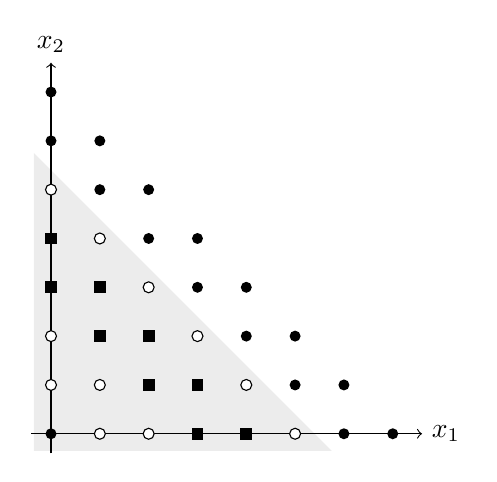
\begin{tikzpicture}[scale=0.62]
\fill[gray!15] (-0.35,-0.35)--(5.75,-0.35)--(-0.35,5.75)--cycle;
\draw[->] (-0.4,0)--(7.6,0) node[right] {$x_1$};
\draw[->] (0,-0.4)--(0,7.6) node[above] {$x_2$};
\foreach \i in {0,...,7}{\foreach \j in {0,...,7}{
 \pgfmathtruncatemacro{\s}{\i+\j}
 \ifnum\s<8
  \ifnum\s=1 \draw[fill=white] (\i,\j) circle (3.2pt);
  \else\ifnum\s=2 \draw[fill=white] (\i,\j) circle (3.2pt);
  \else\ifnum\s=5 \draw[fill=white] (\i,\j) circle (3.2pt);
  \else\ifnum\s=3 \fill (\i-0.12,\j-0.12) rectangle (\i+0.12,\j+0.12);
  \else\ifnum\s=4 \fill (\i-0.12,\j-0.12) rectangle (\i+0.12,\j+0.12);
  \else \fill (\i,\j) circle (3.2pt);
  \fi\fi\fi\fi\fi
 \fi}}
\end{tikzpicture}
\caption{The $T$-graded GNS for $T=\langle3,4\rangle$ and $d=2$, so $F=5$ and
the gaps are the points of total degree $1$, $2$ and $5$ (open circles). The
shaded triangle is $C(S)$, the points of total degree at most $5$, with
$c(S)=21$. The atoms are the $9$ points of total degree $3$ and $4$ (squares);
the filled circles are the other elements of $S$;
$N(S)$ consists of the origin and these atoms, so $n(S)=10$, and
$e(S)\,n(S)=90\ge42=d\,c(S)$.}
\label{fig:example}
\end{figure}

\section{Dimension at least three}\label{sec:high}

\begin{lemma}\label{lem:edim}
For $d\ge3$, $\Bd{d}{a}+\Bd{d}{b}\ge F+d^2+d-1$.
\end{lemma}

\begin{proof}
For $d=3$, $\Bd{3}{t}=(t+1)(t+2)/2$, and a direct expansion gives
\[
\Bd{3}{a}+\Bd{3}{b}-F=\tfrac12(a-b)^2+\tfrac52(a+b)+2\ \ge\ 15\ >\ 11 ,
\]
the minimum being attained at $(a,b)=(2,3)$. Passing from $d$ to $d+1$, Pascal's
rule gives $\Bd{d+1}{t}-\Bd{d}{t}=\Bd{d+1}{t-1}\ge \Bd{d+1}{1}=d+1$ for every
$t\ge2$. So the left side grows by at least $2(d+1)$, which is exactly the growth
of the right side.
\end{proof}

\begin{proposition}\label{prop:high}
For $d\ge3$,
\[
d\binom{F+d}{d}\ \le\ \bigl(\Bd{d}{a}+\Bd{d}{b}\bigr)\,\Bd{d}{F-1}.
\]
Consequently $d\,c(S)\le e(S)\,\Bd{d}{F-1}\le e(S)\,n(S)$.
\end{proposition}

\begin{proof}
Two applications of the identity $k\binom{m}{k}=m\binom{m-1}{k-1}$ give
\[
F\,d\binom{F+d}{d}=(F+d)(F+d-1)\,\Bd{d}{F-1}.
\]
Since $F\ge1$,
\[
(F+d)(F+d-1)=F(F+2d-1)+d(d-1)\le F(F+2d-1)+Fd(d-1)=F(F+d^2+d-1),
\]
so $d\binom{F+d}{d}\le (F+d^2+d-1)\,\Bd{d}{F-1}$, and Lemma~\ref{lem:edim}
gives the inequality. By Proposition~\ref{prop:invariants}, $c(S)=\binom{F+d}{d}$
and $e(S)=\Bd{d}{a}+\Bd{d}{b}$; and since $F-1\in T$ (Lemma~\ref{lem:reflect}), the
whole layer $L_d(F-1)$ lies in $N(S)$, so $\Bd{d}{F-1}\le n(S)$.
\end{proof}

\noindent In comparison, the layer used in~\cite[Theorem~5.6]{bcd} has total
degree $s\ge F-(a-1)$, and the proof there bounds $\Bd{d}{s}$ from below by
$2^{1-d}\binom{F+d-1}{d-1}$ and $g(S)$ from above; the loss of the factor
$2^{d-1}$ is what~\eqref{eq:bcd} compensates. The ratio
$d\,c(S)/\Bd{d}{F-1}=(F+d)(F+d-1)/F$ is less than $F+d^2+d$, and
Lemma~\ref{lem:edim} shows that $e(S)$ is at least that large for every $a$
and~$b$.

\section{Dimensions one and two}\label{sec:low}

\begin{proposition}\label{prop:low}
For $d\in\{1,2\}$, $d\,c(S)\le e(S)\,n(S)$; for $d=1$ equality holds.
\end{proposition}

\begin{proof}
Let $k=(F+1)/2$, the number of elements of $T$ in $[0,F]$
(Lemma~\ref{lem:reflect}). For $d=1$ we have $\Bd{1}{t}=1$, so $c(S)=F+1$,
$n(S)=k$ and $e(S)=2$, and $e(S)\,n(S)=F+1=c(S)$.

For $d=2$ we have $\Bd{2}{t}=t+1$, $e(S)=a+b+2$ and $2c(S)=(F+1)(F+2)=2k(2k+1)$.
The $k$ elements $t_1<\dots<t_k$ of $T$ in $[0,F]$ are distinct non-negative
integers, so
$n(S)=\sum_i(t_i+1)\ge 1+2+\dots+k=k(k+1)/2$. If $(a,b)\ne(2,3)$ then
$e(S)\ge 8$, and $e(S)\,n(S)\ge 4k(k+1)\ge 2k(2k+1)$. If $(a,b)=(2,3)$ then
$F=1$, $e(S)=7$, $n(S)=1$ and $2c(S)=6$.
\end{proof}

\noindent The case $d=2$ is~\cite[Theorem~5.5]{bcd}, where $n(S)$ and $g(S)$ are
computed exactly; the argument above is shorter but gives only the inequality.
The equality for $d=1$ is not part of the Lean statements, which state only the
inequality.

\begin{proof}[Proof of Theorem~\ref{thm:main}]
Part~(i) follows from Proposition~\ref{prop:invariants}(a),(b), parts (ii) and
(iii) are Proposition~\ref{prop:invariants}(c), and part (iv) follows from
Propositions~\ref{prop:high} and~\ref{prop:low}, using the identifications
$|C|=c(S)$, $|C\cap S|=n(S)$ and $|A|=\Bd{d}{a}+\Bd{d}{b}$ of
Proposition~\ref{prop:invariants}.
\end{proof}

{\sloppy
\section{Formal verification}\label{sec:lean}

Theorem~\ref{thm:main} is formally verified in Lean~4 (version 4.34.1) with
Mathlib~\cite{mathlib} (commit \texttt{d13f23b7}). The $9$ files are in
version~\repoversion{} of the repository~\cite{repo}, directory
\texttt{lean/Research/TaskP/GradedWilf/}.

\paragraph{The statement.}
The statement file \texttt{Challenge.lean} contains only definitions and the
statement, no proofs. In ASCII transliteration (the \texttt{import},
\texttt{namespace} and \texttt{end} lines and the one-line docstring of
\texttt{Wilf} omitted; the file itself uses Unicode, e.g.\ $\mathbb N$, $\sum$,
$\in$, $\notin$, $\ne$, $\subseteq$ and $\cap$):
{\footnotesize
\begin{verbatim}
abbrev Point (d : Nat) := Fin d -> Nat
def degree {d : Nat} (x : Point d) : Nat := sum i, x i
def scalar (a b : Nat) : AddSubmonoid Nat := AddSubmonoid.closure {a, b}
def graded (a b d : Nat) : Set (Point d) := {x | degree x in scalar a b}
def belowGaps {d : Nat} (S : Set (Point d)) : Set (Point d) :=
  {x | exists h, h notin S /\ x <= h}
def atoms {d : Nat} (S : Set (Point d)) : Set (Point d) :=
  {x | x in S /\ x != 0 /\ forall y in S, forall z in S, x = y + z -> y = 0 \/ z = 0}
def Wilf : Prop :=
  forall a b d : Nat, 2 <= a -> a < b -> a.Coprime b -> 0 < d ->
    let S := graded a b d
    let C := belowGaps S
    let A := atoms S
    C.Finite /\ A.Finite /\
    (AddSubmonoid.closure A : Set (Point d)) = S /\
    (forall G : Set (Point d), (AddSubmonoid.closure G : Set (Point d)) = S -> A subset G) /\
    d * C.ncard <= A.ncard * (C inter S).ncard
\end{verbatim}}
\noindent Here \texttt{Point d}, the functions from $\{0,\dots,d-1\}$ to $\N$,
is $\N^d$, and \texttt{x <= h} is Mathlib's order on functions, which is the
coordinatewise order. \texttt{degree x} is $|x|$, \texttt{scalar a b} is the
submonoid of $\N$ generated by $a$ and $b$, that is $T=\langle a,b\rangle$, and
\texttt{graded a b d} is the $T$-graded GNS of~\cite[Definition~4.1]{cn}.
\texttt{belowGaps S} is the set $C(S)$, with the gaps taken as the true
complement of $S$ in $\N^d$, so \texttt{C inter S} is $N(S)$. \texttt{atoms S}
is the set $A$ of atoms, and \texttt{AddSubmonoid.closure G} is the monoid
generated by $G$, i.e.\ the set of finite sums of elements of $G$, as in the
definition of a generating set in~\cite[§2]{cn}. \texttt{ncard} is the number of
elements of a set, with the value $0$ for an infinite set. \texttt{Wilf} is
Theorem~\ref{thm:main}: the first two conjuncts are (i), and the other three are
(ii), (iii) and (iv).

The final reviewer (see the last section) checked three points.
(1)~\emph{Why the atom count is $e(S)$.} The source defines $e(S)$ as the size of
the unique minimal system of generators~\cite[§2]{cn}. The target does not
assume a formula for it: it proves that $A$ generates $S$ and that every
generating set contains $A$, which makes $A$ that unique minimal system, as in
the proof of Corollary~\ref{cor:wilf}; so \texttt{A.ncard} is $e(S)$.
(2)~\emph{Why the counts are true cardinalities.} Since \texttt{ncard} would
return $0$ for an infinite set, the target asserts that $C$ and $A$ are finite;
$C\cap S\subseteq C$ is then finite too. So the three \texttt{ncard} values are
the actual numbers $c(S)$, $e(S)$ and $n(S)$, and the inequality cannot hold
for the trivial reason that a count is $0$. Finiteness of $C$ also gives
finiteness of the gap set, so $S$ is indeed a GNS. In its own audit file the
reviewer proved in Lean that for $(a,b,d)=(3,4,3)$ the three numbers are
$56$, $25$ and $26$. (3)~\emph{Quantifiers.} The target covers every $d\ge1$
and every pair of coprime integers $2\le a<b$, hence every two-generated
numerical semigroup, with no further hypotheses, and the inequality is
$d\,c(S)\le e(S)\,n(S)$, as in~\cite{cdffpu}. Because of (ii) and (iii) of
Theorem~\ref{thm:main}, the target is stronger than the bare inequality.

\paragraph{Review and freezing.}
\texttt{Challenge.lean} was reviewed against~\cite{cn} by a Codex agent that had
not written it, and frozen, by recording its SHA-256 hash, on 20 November 2026
at 18:04~UTC. The development logs record no compilation of a proof file before
that time, and the file was not changed afterwards.

\paragraph{The proofs.}
In \texttt{Proof.lean}, \texttt{Proof.Wilf} obtains the finiteness, generation
and minimality statements from the lemmas listed in Table~\ref{tab:lean}, rewrites
the three cardinalities with the formulas of
Proposition~\ref{prop:invariants}, and then uses \texttt{high\_\allowbreak wilf}
together with the layer $F-1$ when $d\ge3$, and
\texttt{low\_\allowbreak wilf} when $d\le2$. Table~\ref{tab:lean} lists the Lean
counterparts of the steps of the written proof (names in the namespace
\texttt{TaskP.GradedWilf}; $F$ is \texttt{frob a b}, $\Bd{d}{t}$ is Mathlib's
\texttt{d.multichoose t}, and the set of $t\le F$ with $t\in T$ is
\texttt{good a b}).

\begin{table}[ht]
\centering\footnotesize
\renewcommand{\arraystretch}{1.18}
\begin{tabular}{@{}>{\raggedright\arraybackslash}p{0.44\textwidth}>{\raggedright\arraybackslash}p{0.52\textwidth}@{}}
\hline
Step of the written proof & Lean (file) \\
\hline
Lemma~\ref{lem:reflect}: Sylvester's theorem &
\texttt{frob\_spec} (\texttt{WilfScalar}), from Mathlib's
\texttt{frobeniusNumber\_pair} \\
Lemma~\ref{lem:reflect}: $1\notin T$, the reflection $t\leftrightarrow F-t$,
and $F-1\in T$ &
\texttt{one\_gap}, \texttt{reflect\_mem}, \texttt{penultimate\_mem}
(\texttt{WilfScalar}) \\
Lemma~\ref{lem:reflect}: $(F+1)/2$ elements of $T$ in $[0,F]$ &
\texttt{twice\_card\_good} (\texttt{WilfLow}) \\
Layers and their sizes $\Bd{d}{t}$, and $\sum_{t\le F}\Bd{d}{t}=\binom{F+d}{d}$ &
\texttt{layer}, \texttt{card\_layer}, \texttt{ball}, \texttt{card\_ball}
(\texttt{WilfLayers}) \\
Proposition~\ref{prop:invariants}(a): $C$ is the set of points of total degree
at most $F$ & \texttt{below\_eq\_ball} (\texttt{WilfLayers}) \\
Proposition~\ref{prop:invariants}(a): the formula for $n(S)$ &
\texttt{good\_count} (\texttt{WilfLow}) \\
Proposition~\ref{prop:invariants}(b): the atoms are the layers $a$ and $b$ &
\texttt{atoms\_eq} (\texttt{WilfAtoms}), with \texttt{take\_degree},
\texttt{split\_scalar}, \texttt{min\_degree}, \texttt{divides\_small} \\
Proposition~\ref{prop:invariants}(c) &
\texttt{atoms\_generate}, \texttt{atoms\_minimal} (\texttt{WilfBasis}) \\
Lemma~\ref{lem:edim} &
\texttt{embedding\_lower} (\texttt{WilfHigh}), with the private
\texttt{mc\_three}, \texttt{mc\_step} \\
$F\,d\binom{F+d}{d}=(F+d)(F+d-1)\Bd{d}{F-1}$ &
private \texttt{slice\_ratio} (\texttt{WilfHigh}) \\
Proposition~\ref{prop:high}, first inequality &
\texttt{high\_wilf} (\texttt{WilfHigh}) \\
Proposition~\ref{prop:low} (inequality only) &
\texttt{low\_wilf} (\texttt{WilfLow}), with \texttt{twice\_sum\_succ} for the
bound $k(k+1)\le 2\sum_i(t_i+1)$ \\
Assembly of Theorem~\ref{thm:main} &
\texttt{Proof.Wilf} (\texttt{Proof}) \\
\hline
\end{tabular}
\caption{Lean counterparts of the steps of the proof.}
\label{tab:lean}
\end{table}

\noindent The test file \texttt{CheckWilf.lean} restates the theorem with the
frozen type (\texttt{check\_\allowbreak Wilf}). The axioms of
\texttt{check\_\allowbreak Wilf} and of \texttt{Proof.Wilf}, printed by
\texttt{CheckWilf.lean}, are exactly \texttt{propext}, \texttt{Classical.choice}
and \texttt{Quot.sound}. No file uses \texttt{sorry}, \texttt{decide},
\texttt{native\_\allowbreak decide}, \texttt{bv\_\allowbreak decide} or an
\texttt{axiom} declaration.

\paragraph{Checks.}
The $9$ files ($6$ proof modules, \texttt{Challenge.lean}, \texttt{Proof.lean}
and \texttt{CheckWilf.lean}) were compiled module by module in two new empty
directories on the author's Mac, with the pinned toolchain and with warnings
treated as errors, on 20 November 2026 (18:21--18:24~UTC), and every module was
replayed with \texttt{leanchecker}; each directory also ran one build of the
whole package. All $38$ commands ($19$ per directory) ended with exit code~$0$,
the \texttt{leanchecker} runs printed nothing, and the two directories produced
identical \texttt{.olean} files. The final reviewer (see the next section)
compiled the $9$ files again, together with a short audit file of its own, in a
third new directory on the author's Mac on 20 November 2026 (18:31--18:34~UTC),
with warnings treated as errors, and replayed every module with
\texttt{leanchecker}; every reviewed module compiled and replayed with exit
code~$0$; a first draft of the audit file contained errors in the reviewer's own
numerical examples and was corrected and recompiled, and no reviewed file was
changed. Mathlib and its dependencies were
taken from a shared prebuilt cache at the pinned commits and were not rechecked;
the \texttt{leanchecker} replays cover the $9$ project modules. In the repository
the files have module names under \texttt{Research.TaskP.GradedWilf} and differ
from the checked files only in their \texttt{import} lines
(\texttt{Challenge.lean} is unchanged). The repository versions were made by a script that changed only the local \texttt{import} lines, and on 20 November 2026 (19:55--20:07~UTC) they were compiled and replayed with \texttt{leanchecker} again, module by module, in two new empty directories on the author's Mac, one after the other, together with the files of three other papers of version~\repoversion{} ($39$ modules in all); there were no warnings, and the two directories produced identical \texttt{.olean} files and the same axiom lists. In the whole-project rebuild of version~\repoversion{} of the repository (on the author's Windows computer, in two passes on 20 and 21 November 2026), these files were compiled and replayed with \texttt{leanchecker} again in pass~2 (21 November 2026), which built the files not included in pass~1 on top of its results; no module needed a second attempt (details in the repository). The
formalization has not been checked with comparator or with an independent
kernel.

\par}

\section*{How this paper was produced}
This work was carried out from 20 to 22 November 2026 (UTC) in a workflow directed by
the author, using OpenAI Codex with the model GPT-6.2-Astra (reasoning level
ultra) and Anthropic Claude Code with the model Claude Opus~5.5. The author asked
for a further search for substantial open problems, and Claude
Code passed this request to Codex at 17:23~UTC. Between 17:23 and 17:53~UTC,
Codex recorded $111$ problems from the literature and wrote proofs for five
candidates; for the problem of this paper, the inequality, computed from the
layer formulas, was checked by exact computation for all $6{,}204$ triples $(a,b,d)$ with $2\le a\le24$, $a<b\le50$, $\gcd(a,b)=1$ and
$1\le d\le12$, and the proof was read by another Codex agent (same model) that had not
taken part in it. The author had asked in advance that the five most important
candidates be formalized at once, without waiting for a choice; this problem
was among the five selected at 18:00~UTC. From then on, Codex agents (same model)
checked the reading of the sources, searched again for prior work, wrote the
statement file, the Lean proof and the written proof, and ran the checks. The
reading of the sources was checked by a Codex agent that had not taken part in
the proof or in drafting the statement, and the statement file was reviewed
before it was frozen by a Codex agent that had written neither the proofs nor
the statement. According to the file timestamps and the development logs, the
proof files were created after the freeze and compiled between 18:07 and
18:18~UTC; they follow the written proof prepared in the search for problems.
After the checks, an independent Claude Code agent (model Claude Opus~5.5) that
had written none of the files gave the final review. It read the three sources
itself~\cite{cdffpu,cn,bcd}, compared the statement file with them, read the
written proof, the proof files and the raw logs of the checks, checked the
invariants by brute-force enumeration and the inequality on $18{,}096$ parameter
triples in Python, and rebuilt the formalization as described above. Its
decision was APPROVE\_FORMAL, with five minor remarks on the written account
(one optional), all taken into account here. Claude Code (Claude Opus~5.5)
checked the sources and wrote this text from Codex's manuscript and the Lean
files. An independent Claude Code agent (model Claude Opus~5.5) that had written none of the files reviewed this paper, and another reviewed the release; their corrections were applied. Throughout, ``we'' refers to this workflow; the reading and
searching described in the paper were done by the agents. Codex agents searched
for prior work on 20 November 2026, in the search for problems and again before
the statement was frozen; they found the partial results of~\cite{bcd}, but no
proof of the inequality for the parameters left open there (details in the
repository). Claude Code searched again on 21 November 2026 (17:54--18:21~UTC; the arXiv, Semantic Scholar, Crossref, DataCite, Zenodo, MathDB, GitHub and repositories of AI-assisted mathematics) and found no new related work and no new version of~\cite{bcd}; that day the citation index OpenAlex refused to list the works citing~\cite{cn} (rate limit). Claude Code searched again on 22 November 2026 (05:39--05:51~UTC), when the OpenAlex lists of citing works refused on 21 November were retrieved, and found nothing new. This reports the coverage of the searches, not
a guarantee that they were complete. The author is not a professional
mathematician. The author has read this paper and, using a side-by-side table, compared its Lean statement with the main theorem, Theorem~\ref{thm:main}. No human mathematician has reviewed this paper. The
correctness of the results rests on the Lean proofs and on the agreement of the
Lean statement with the conjecture of~\cite{cdffpu} for the class of~\cite{cn};
the written proofs are given for the reader. AI systems are not authors of this
paper; the author takes full responsibility for its content.

\medskip
\noindent Thanks are due to Carmelo Cisto and Francesco Navarra for the
question.

{\small
\begin{thebibliography}{9}
\setlength{\itemsep}{1pt}
\bibitem{bcd} O.~P. Bhardwaj, C.~Cisto and P.~Deshpande, Structure of gaps and
generalized Wilf's conjecture, arXiv:2611.20086v1, 2026.
\bibitem{cdffpu} C.~Cisto, M.~DiPasquale, G.~Failla, Z.~Flores, C.~Peterson and
R.~Utano, A generalization of Wilf's conjecture for generalized numerical
semigroups, \emph{Semigroup Forum} 101 (2020), no.~2, 303--325,
\url{https://doi.org/10.1007/s00233-020-10085-7}; arXiv:1909.13120.
\bibitem{cn} C.~Cisto and F.~Navarra, On some classes of generalized numerical
semigroups, \emph{An. Ştiinţ. Univ. ``Ovidius'' Constanţa Ser. Mat.} 33
(2025), no.~1, 153--175, \url{https://doi.org/10.2478/auom-2025-0008};
arXiv:2212.12467v1 (2022).
\bibitem{repo} H.~Dong, \emph{ai4math-results}, repository,
\url{https://github.com/Horace-Maxwell/ai4math-results}, version~\repoversion{}
(2026); archived at Zenodo under the concept DOI
\url{https://doi.org/10.5281/zenodo.22970254}.
\bibitem{mathlib}
The mathlib Community, The Lean mathematical library, in \emph{Proc.\ 9th ACM
SIGPLAN Int.\ Conf.\ Certified Programs and Proofs} (CPP '20), ACM, 2020,
\url{https://doi.org/10.1145/3372885.3373824}.
\bibitem{rg} J.~C. Rosales and P.~A. García-Sánchez, \emph{Numerical
Semigroups}, Developments in Mathematics~20, Springer, New York, 2009,
\url{https://doi.org/10.1007/978-1-4419-0160-6}.
\bibitem{wilf} H.~S. Wilf, A circle-of-lights algorithm for the
``money-changing problem'', \emph{Amer. Math. Monthly} 85 (1978), no.~7,
562--565, \url{https://doi.org/10.1080/00029890.1978.11994639}.
\end{thebibliography}}
\end{document}
